\documentclass[9pt]{beamer}


\usepackage[utf8x]{inputenc}
\usepackage{beamerthemeOxygen}
\usepackage{MinionPro}
\usefonttheme{serif} 
%\setbeamerfont{structure}{family=\rmfamily} 

\newcommand{\page}[1]{\frame{#1}}

\usepackage{graphicx}
\usepackage{pstricks}
\usepackage{color}
\usepackage{listings}
\usepackage{amsmath}
\usepackage{amsfonts}
\usepackage{amssymb}
\usepackage{amsthm}
\usepackage{listings}
\usepackage[vlined,linesnumbered]{algorithm2e}
\usepackage{xspace}  % to allow for text macros that don't eat space 
\newcommand{\field}[1]{\mathbb{#1}}
\newcommand{\ideal}[1]{\langle #1 \rangle}
\newcommand{\PRESENT}{\textsc{Present}\xspace}

\newcommand{\M}[1]{\ensuremath{\textsc{M}(#1)\xspace}}
\newcommand{\LT}[1]{\ensuremath{\textsc{LT}(#1)\xspace}}
\newcommand{\LM}[1]{\ensuremath{\textsc{LM}(#1)\xspace}}
\newcommand{\LC}[1]{\ensuremath{\textsc{LC}(#1)\xspace}}
\newcommand{\LCM}[1]{\ensuremath{\textsc{LCM}(#1)\xspace}}

\newtheorem{thm}{Theorem}[section]

\newcommand{\dred}{\color{oxygenorange}\bf}
\newcommand{\dblue}{\color{oxygenblue}\bf}
\newcommand{\dgray}{\color{oxygengray}\bf}


\title{Algebraic Techniques in Cryptanalysis}
\subtitle{of Block Ciphers with a bias towards \texorpdfstring{Gröbner}{Groebner} bases}
\author{Martin R.\ Albrecht}

\institute{Team SALSA, UPMC, Paris 6, \dots}
\date{June 2nd, 2011 @ ECrypt 2 PhD Summer school, Albena, Bulgaria}
\AtBeginSection[]
{
   \begin{frame}
       \frametitle{Outline}
       \tableofcontents[currentsection]
   \end{frame}
}

\lstdefinelanguage{Sage}[]{Python}
{morekeywords={True,False,sage},
sensitive=true}

\definecolor{Gray}{gray}{.5}

\lstset{frame=none,
          showtabs=False,
          showspaces=False,
          showstringspaces=False,
          commentstyle={\color{oxygenorange}},
          keywordstyle={\color{oxygenblue}\bfseries},
          stringstyle ={\color{Gray}},
          language = Sage,
          basicstyle={\footnotesize\ttfamily}
          }

\begin{document}

\begin{frame}

\titlepage
\end{frame}

\begin{frame}
\frametitle{Outline}
\tableofcontents
\end{frame}

\section{Introduction}

\begin{frame}
\frametitle{What are Algebraic Attacks?} 

\begin{enumerate}
 \item Algebraic attacks model a cryptographic primitive (such as a block cipher) as a system of equations.
 \item Then, by applying (algebraic) transformations to these equations they (attempt to) recover information about the secret of the primitive (the key).
\end{enumerate}

\begin{block}{}
Hence, they are quite different in spirit from statistical techniques such as linear and differential cryptanalysis.
\end{block}

\end{frame}


\begin{frame}
\frametitle{A Polemic History of Algebraic Attacks}
\textbf{1959} -- the ``prophecy''
\begin{quote}
``Thus, if we could show that solving a certain system requires at least as much work as solving a system of
simultaneous equations in a large number of unknowns, of a complex type, then we would have a lower bound of sorts for
the work characteristic.'' 
\end{quote}
\begin{flushright}
\vspace{-2em}
-- Claude Shannon
\end{flushright}

\textbf{2002} -- the breakthrough
\begin{quote}
Crucial Cipher Flawed, Cryptographers Claim -- Two cryptographers say that the new Advanced Encryption Standard, [\dots] has a hole in it. Although some of their colleagues doubt the validity of their analysis, the cryptographic community is on edge, wondering whether the new cipher can withstand a future assault.
\end{quote}
\begin{flushright}
\vspace{-2em}
-- Science Magazine
\end{flushright}

\textbf{2011} -- the disillusion

\vspace{0.8em}

\begin{tabular}{ll}
\hspace{0.05cm} & Not a single proper \emph{block cipher} has been broken using \textit{pure} algebraic techniques\\ & faster than with other techniques.
\end{tabular}
\end{frame}

\begin{frame}
\frametitle{So, why bother?}

Algebraic techniques 
\begin{enumerate}
 \item have been proven powerful against some stream ciphers and public key schemes,
 \item provide a unified attack methodology for various areas of cryptography,
 \item may be one of the few choices if very few plaintext-ciphertext pairs are available,
 \item may prove useful under more relaxed attack settings (many plaintexts \dots),
 \item become more relevant as focus shifts toward (very) lightweight constructions,
 \item can be combined with other techniques (differential, side-channels, \dots),
 \item are fun \dots well, to some anyway!
\end{enumerate}
 
\end{frame}


\section{Equations}

\begin{frame}[allowframebreaks]
\frametitle{SP-Networks} 

We construct an equation system for the block cipher \PRESENT, which

\begin{itemize}
 \item is a substituion-permutation network,
 \item has a block size of 64 bits,
 \item either takes 80-bit or 128-bit keys (\PRESENT-80 and \PRESENT-128 resp.)
 \item has 31 rounds (shorter variants are denoted by \PRESENT-\{80,128\}-$Nr$),
 \item is conceptually simple, and
 \item has been extensively studied (differential, linear, side-channels, higher-order differential, algebraic).
\end{itemize}

\begin{small}
\begin{thebibliography}{present}
\bibitem{present}
Andrey Bogdanov, Lars~R. Knudsen, Gregor Leander, Christof Paar, Axel
  Poschmann, Matthew J.~B. Robshaw, Yannick Seurin, and C.~Vikkelsoe.
\newblock {PRESENT}: An ultra-lightweight block cipher.
\newblock In {\em Cryptographic Hardware and Embedded Systems - CHES 2007},
  volume 7427 of {\em Lecture Notes in Computer Science}, pages 450--466,
  Berlin, Heidelberg, New York, 2007. Springer Verlag.
\end{thebibliography}
\end{small}
\framebreak

\begin{center}
 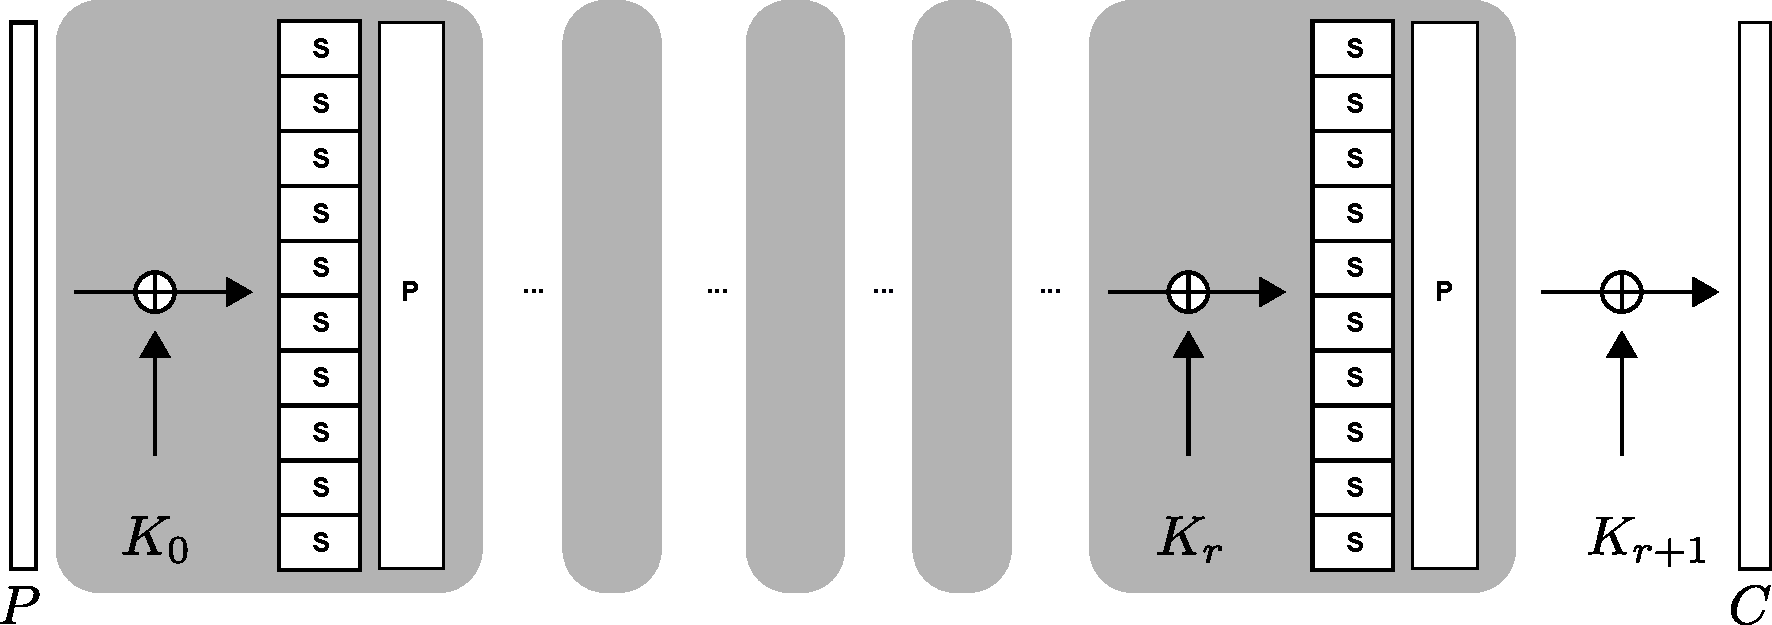
\includegraphics[width=1.0\textwidth]{./spn-scheme.pdf}
 % spn-scheme.pdf: 842x595 pixel, 72dpi, 29.70x20.99 cm, bb=0 0 842 595
\end{center}
\end{frame}

\begin{frame}
\frametitle{Key Addition and the Permutation Layer}

\begin{itemize}
  \item \emph{Key addition} is easy, if $X_i$ is a bit before key addition and $Y_i$ is a bit after key addition, we write:
\[Y_i + X_i + K_i (=0).\]
  \item the \emph{Permutation layer} is just a permutation of wires given by the rule
\[s \cdot j + i \Rightarrow  B \cdot i + j \textnormal{ for } 0 \leq j < 16 \textnormal{ and } 0 \leq i < 4,\] hence we simply rename variables.
\end{itemize}

\begin{block}{}
In general the permuation layer gives rise to linear equations. 
\end{block}


\end{frame}

\begin{frame}[allowframebreaks,fragile]
\frametitle{S-Box}
\begin{columns}

\column{0.5\textwidth}

The S-box is a non-linear operation. However, finding equations is still easy.

\vspace{1em}

As an example consider the 3-bit (since it fits on the slides) S-box 

$$[7,6,0,4,2,5,1,3].$$

\vspace{1em}

Construct the matrix on the right and perform fraction-free Gaussian elimination on it (fitting a linear model).

\column{0.5\textwidth}
\begin{scriptsize}
\begin{align*}
\begin{array}{rrrrrrrrrr}
0\ & 1 & 2\  & 3 & 4\  & 5 & 6 & 7 & \ \ \ \ \ \ \ \ \ \ \\
\end{array}\\
\left(\begin{array}{rrrrrrrrr}
1 & 1 & 1 & 1 & 1 & 1 & 1 & 1 & 1 \\
0 & 0 & 0 & 0 & 1 & 1 & 1 & 1 & x_{0} \\
0 & 0 & 1 & 1 & 0 & 0 & 1 & 1 & x_{1} \\
0 & 1 & 0 & 1 & 0 & 1 & 0 & 1 & x_{2} \\
1 & 1 & 0 & 1 & 0 & 1 & 0 & 0 & y_{0} \\
1 & 1 & 0 & 0 & 1 & 0 & 0 & 1 & y_{1} \\
1 & 0 & 0 & 0 & 0 & 1 & 1 & 1 & y_{2} \\
0 & 0 & 0 & 0 & 0 & 0 & 1 & 1 & x_{0} x_{1} \\
0 & 0 & 0 & 0 & 0 & 1 & 0 & 1 & x_{0} x_{2} \\
0 & 0 & 0 & 0 & 0 & 1 & 0 & 0 & x_{0} y_{0} \\
0 & 0 & 0 & 0 & 1 & 0 & 0 & 1 & x_{0} y_{1} \\
0 & 0 & 0 & 0 & 0 & 1 & 1 & 1 & x_{0} y_{2} \\
0 & 0 & 0 & 1 & 0 & 0 & 0 & 1 & x_{1} x_{2} \\
0 & 0 & 0 & 1 & 0 & 0 & 0 & 0 & x_{1} y_{0} \\
0 & 0 & 0 & 0 & 0 & 0 & 0 & 1 & x_{1} y_{1} \\
0 & 0 & 0 & 0 & 0 & 0 & 1 & 1 & x_{1} y_{2} \\
0 & 1 & 0 & 1 & 0 & 1 & 0 & 0 & x_{2} y_{0} \\
0 & 1 & 0 & 0 & 0 & 0 & 0 & 1 & x_{2} y_{1} \\
0 & 0 & 0 & 0 & 0 & 1 & 0 & 1 & x_{2} y_{2} \\
1 & 1 & 0 & 0 & 0 & 0 & 0 & 0 & y_{0} y_{1} \\
1 & 0 & 0 & 0 & 0 & 1 & 0 & 0 & y_{0} y_{2} \\
1 & 0 & 0 & 0 & 0 & 0 & 0 & 1 & y_{1} y_{2}
\end{array}\right)
\end{align*}
\end{scriptsize}
\end{columns}
\begin{scriptsize}
\begin{align*}
\left(\begin{array}{rrrrrrrrr}
1 & 0 & 0 & 0 & 0 & 0 & 0 & 0 & x_{0} y_{0} + x_{1} + x_{2} + y_{0} + y_{1} + 1\\
0 & 1 & 0 & 0 & 0 & 0 & 0 & 0 & x_{0} y_{0} + x_{0} + x_{1} + y_{2} + 1 \\
0 & 0 & 1 & 0 & 0 & 0 & 0 & 0 & x_{0} y_{0} + x_{0} + y_{0} + 1 \\
0 & 0 & 0 & 1 & 0 & 0 & 0 & 0 & x_{0} y_{0} + x_{0} + x_{2} + y_{1} + y_{2} \\
0 & 0 & 0 & 0 & 1 & 0 & 0 & 0 & x_{0} y_{0} + x_{0} + x_{1} + x_{2} + y_{0} + y_{1} + y_{2} + 1 \\
0 & 0 & 0 & 0 & 0 & 1 & 0 & 0 & x_{0} y_{0} \\
0 & 0 & 0 & 0 & 0 & 0 & 1 & 0 & x_{0} y_{0} + x_{2} + y_{0} + y_{2} \\
0 & 0 & 0 & 0 & 0 & 0 & 0 & 1 & x_{0} y_{0} + x_{1} + y_{1} + 1 \\
0 & 0 & 0 & 0 & 0 & 0 & 0 & 0 & \mathbf{x_{0} x_{2} + x_{1} + y_{1} + 1} \\
0 & 0 & 0 & 0 & 0 & 0 & 0 & 0 & \mathbf{x_{0} x_{1} + x_{1} + x_{2} + y_{0} + y_{1} + y_{2} + 1} \\
0 & 0 & 0 & 0 & 0 & 0 & 0 & 0 & \mathbf{x_{0} y_{1} + x_{0} + x_{2} + y_{0} + y_{2}} \\
0 & 0 & 0 & 0 & 0 & 0 & 0 & 0 & \mathbf{x_{0} y_{0} + x_{0} y_{2} + x_{1} + x_{2} + y_{0} + y_{1} + y_{2} + 1} \\
0 & 0 & 0 & 0 & 0 & 0 & 0 & 0 & \mathbf{x_{1} x_{2} + x_{0} + x_{1} + x_{2} + y_{2} + 1} \\
0 & 0 & 0 & 0 & 0 & 0 & 0 & 0 & \mathbf{x_{0} y_{0} + x_{1} y_{0} + x_{0} + x_{2} + y_{1} + y_{2}} \\
0 & 0 & 0 & 0 & 0 & 0 & 0 & 0 & \mathbf{x_{0} y_{0} + x_{1} y_{1} + x_{1} + y_{1} + 1} \\
0 & 0 & 0 & 0 & 0 & 0 & 0 & 0 & \mathbf{x_{1} y_{2} + x_{1} + x_{2} + y_{0} + y_{1} + y_{2} + 1} \\
0 & 0 & 0 & 0 & 0 & 0 & 0 & 0 & \mathbf{x_{0} y_{0} + x_{2} y_{0} + x_{1} + x_{2} + y_{1} + 1} \\
0 & 0 & 0 & 0 & 0 & 0 & 0 & 0 & \mathbf{x_{2} y_{1} + x_{0} + y_{1} + y_{2}} \\
0 & 0 & 0 & 0 & 0 & 0 & 0 & 0 & \mathbf{x_{2} y_{2} + x_{1} + y_{1} + 1} \\
0 & 0 & 0 & 0 & 0 & 0 & 0 & 0 & \mathbf{y_{0} y_{1} + x_{0} + x_{2} + y_{0} + y_{1} + y_{2}} \\
0 & 0 & 0 & 0 & 0 & 0 & 0 & 0 & \mathbf{y_{0} y_{2} + x_{1} + x_{2} + y_{0} + y_{1} + 1} \\
0 & 0 & 0 & 0 & 0 & 0 & 0 & 0 & \mathbf{y_{1} y_{2} + x_{2} + y_{0}}
\end{array}\right)              
\end{align*}
\end{scriptsize}


\framebreak

If you cannot be bothered to do that yourself, use Sage \begin{small}(\url{http://www.sagemath.org})\end{small}:

\begin{lstlisting}
sage: S = mq.SBox(7,6,0,4,2,5,1,3)
sage: S.polynomials()
[x0*x2 + x1 + y1 + 1, 
 x0*x1 + x1 + x2 + y0 + y1 + y2 + 1, 
 x0*y1 + x0 + x2 + y0 + y2, 
 x0*y0 + x0*y2 + x1 + x2 + y0 + y1 + y2 + 1, 
 x1*x2 + x0 + x1 + x2 + y2 + 1, 
 x0*y0 + x1*y0 + x0 + x2 + y1 + y2, 
 x0*y0 + x1*y1 + x1 + y1 + 1,
 x1*y2 + x1 + x2 + y0 + y1 + y2 + 1,
 x0*y0 + x2*y0 + x1 + x2 + y1 + 1,
 x2*y1 + x0 + y1 + y2,
 x2*y2 + x1 + y1 + 1,
 y0*y1 + x0 + x2 + y0 + y1 + y2,
 y0*y2 + x1 + x2 + y0 + y1 + 1,
 y1*y2 + x2 + y0]
\end{lstlisting}

If we post-process these polynomials (\lstinline{groebner=True}), we get 21 quadratic equations and one cubic equation for the S-Box which have a nice algebraic structure.

\end{frame}

\begin{frame}[fragile]
\frametitle{Putting it all together} 

\begin{itemize}
 \item We have equations for the $S$ layer, $P$ layer and the key addtion.
 \item The key schedule is similar and has one/two S-boxes. 
 \item For each round we introduce $2 \cdot 64$ new state variables for the $S$ layer.
 \item Adding key schedule and key variables we get $132 \cdot Nr +80$ variables
 \item On ther other hand, we get $(22 ⋅ 16 + 22 + 64)Nr + 64$ equations
\end{itemize}

\begin{lstlisting}
# from http://bitbucket.org/malb/algebraic_attacks/present.py
sage: attach present.py
sage: p = PRESENT(Nr=31)
sage: F,s = p.polynomial_system(); F
Polynomial System with 13642 Polynomials in 4172 Variables
\end{lstlisting}

\begin{block}{}
Solving this system means recovering the key \dots
\end{block}
\end{frame}


\section{Solvers}

\begin{frame}
\frametitle{Solver Families} 

\vfill

In cryptography there are four families of algorithms which are usually used for solving systems of equations.

\vfill

In order of popularity for block ciphers:
\begin{enumerate}
 \item SAT solvers: MiniSat2, CryptoMiniSat, (Raddum-Semaev, MRHS), \dots
 \item Gröbner basis methods: Buchberger's algorithm, F$_4$, F$_5$, \dots
 \item Mixed Integer (Linear) Solvers: SCIP, CPLEX, Gurobi, \dots
 \item Algebraic higher-order differential: AIDA, Cube attack, Cube Tester, \dots
\end{enumerate}

\vfill

It is very useful to understand a bit how these solvers work.

\vfill

\begin{block}{}
``We put our equations into \textsc{Magma} and it ran out of memory'' is not a valid analysis.
\end{block}

\vfill

\end{frame}


\begin{frame}[allowframebreaks,fragile]
\frametitle{Gröbner Bases}
\framesubtitle{for Cryptographers} 

\begin{itemize}
 \item $P = \field{F}_q[x_0,\dots,x_{n-1}]$.
 \item $\field{F}_q$ is a finite field of order $q$.
 \item $\mathcal{I}$ is an ideal $ \subset P$. That is, 
  \begin{itemize}
  \item $f,g \in \mathcal{I} \longrightarrow f + g \in \mathcal{I}$ and 
  \item $f \in P, g \in \mathcal{I} \longrightarrow f \cdot g \in \mathcal{I}.$
  \end{itemize}
 
 \item $\ideal{f_0,\dots,f_{m-1}}$ is the ideal spanned by $f_0,\dots,f_{m-1}$.
\begin{lstlisting}
sage: P.<x,y,z> = PolynomialRing(GF(127),order='deglex')
sage: I = ideal(x*y + z, y^3 + 1, z^2 - x*5 - 1)
sage: (x*y + z) + (y^3 + 1) in I
True
sage: x*z*(z^2 - x*5 - 1) in I
True
\end{lstlisting}
\framebreak 
 \item A term order decides how we compare monomials, e.g., is $xy$ or $y^3$ bigger (degree or variable first)?
\begin{lstlisting}
sage: P.<x,y,z> = PolynomialRing(GF(127),order='lex')
sage: x*y > y^3
True
sage: P.<x,y,z> = PolynomialRing(GF(127),order='deglex')
sage: x*y > y^3
False
\end{lstlisting}
 \item $\M{f}$ is the set of all monomials in $f$.
 \item $\LM{f}$ is the leading or largest monomial in $f$.
\begin{lstlisting}
sage: P.<x,y,z> = PolynomialRing(GF(127),order='deglex')
sage: f = x*y + x + 3
sage: f.lm()
x*y
sage: f.monomials()
[x*y, x, 1]
\end{lstlisting}
\end{itemize}

\framebreak

\begin{definition}[Gr\"obner Basis]
Let $\mathcal{I}$ be an ideal of $\field{F}[x_0,\dots,x_{n-1}]$ and fix a monomial ordering. A finite subset $$G = \{g_0 ,\dots , g_{m-1} \} \subset \mathcal{I}$$  is said to be a \emph{Gr\"obner basis} of $\mathcal{I}$ if for any $f \in \mathcal{I}$ there exists $g_i \in G$ such that $$\LM{g_i} \mid \LM{f}.$$
\end{definition}

\vspace{1em}

Among other things Gröbner bases allow to solve (non-linear) systems of equations. However, they are much more powerful objects than just that, as we will discuss at the end of this talk.

\vspace{1em}

\begin{block}{Note}
Gröbner bases generalise greatest common divisors over $\field{F}[x]$ and row echelon forms over $\field{F}^n$.
\end{block}

\framebreak

As a warm-up, consider a linear system of equations over $\field{F}_{127}[x,y,z]$.

\begin{columns}
\column{0.5\textwidth}
\begin{align*}
f &= 26y + 52z + 62 = 0\\
g &= 54y + 119z + 55 = 0\\
h &= 41x + 91z + 13 = 0
\end{align*}
\begin{align*}
f' &= x + 29 = 0\\
g' &= y + 38 = 0\\
h' &= z + 75 = 0
\end{align*}
\column{0.5\textwidth}
\begin{align*}
\left(\begin{array}{rrrr}
0 & 26 & 52 & 62 \\
0 & 54 & 119 & 55 \\
41 & 0 & 91 & 13
\end{array}\right)
\end{align*}
\begin{align*}
\left(\begin{array}{rrrr}
1 & 0 & 0 & 29 \\
0 & 1 & 0 & 38 \\
0 & 0 & 1 & 75
\end{array}\right)
\end{align*}
\end{columns}

\vspace{1em}

Thus, $x = -29$, $y = - 38$ and $z = - 75$ is a solution.

\vspace{1em}

\begin{block}{Note}
Gaussian elimination iteratively reduces the leading terms: $\LM{h} = x \Rightarrow \LM{h'} = z$.
\end{block}

\framebreak

Now consider two polynomials in $\field{F}_{127}[x,y,z]$ with term ordering \textbf{deglex}.

\begin{columns}
\column{0.5\textwidth}
\begin{align*}
f &= x^2 + 2xy - 2y^2 + 14z^2 + 22z\\
g &= x^2 + xy + y^2 + z^2 + x + 2z
\end{align*}
\begin{align*}
f &= x^2 + 4 y^2  -12 z^2 + 2 x - 18 z \\
g'&= x y + -3 y^{2} + 13 z^{2} - x + 20 z
\end{align*}
\column{0.5\textwidth}
\begin{align*}
\left(\begin{array}{rrrrrr}
1 & 2 & -2 & 14 & 0 & 22 \\
1 & 1 &  1 &  1 & 1 &  2
\end{array}\right)
\end{align*}
\begin{align*}
\left(\begin{array}{rrrrrr}
1 & 0 &  4 & -12 &  2 & -18 \\
0 & 1 & -3 &  13 & -1 &  20
\end{array}\right)
\end{align*}
\end{columns}

\vspace{1em}

\begin{block}{}
Gaussian elimination still ``reduces'' the system.
\end{block}


\framebreak

This approach fails for
\begin{align*}
f &= \mathbf{x^2} - 2\mathbf{xy} - 2y^2 + 14z^2,\\
g &= \mathbf{x} + y + 2z.
\end{align*}
since $x$ is not a monomial of $f$. 

\vspace{1em}

However, $x$ divides two monomials of $f$: $x^2$ and $xy$. 

\vspace{1em}

To account for those include multiples $m \cdot g$ of $g$ such that $$\LM{m \cdot g} = m \cdot \LM{g} \in \M{f}.$$

\framebreak

\begin{columns}
\column{0.4\textwidth}
\begin{align*}
f &= x^2 - 2xy - 2y^2 + \dots \\
x \cdot g &= \mathbf{x^{2}} + x y \dots\\
y \cdot g &= \mathbf{xy} + y^{2} + \dots\\
g &= x + y + 2z
\end{align*}
\begin{align*}
f' &= x^{2} + 4 y z + 14 z^{2},\\
h_1 &= \mathbf{x y} + 2 x z + -4 y z - \dots,\\
h_2 &= \mathbf{y^{2}} -2 x z + 6 y z + \dots,\\
g &= x + y + 2 z
\end{align*}
\column{0.6\textwidth}
\begin{align*}
\left(\begin{array}{rrrrrrrrr}
1 & -2 & -2 & 0 & 0 & 14 & 0 & \dots \\
1 & 1 & 0 & 2 & 0 & 0 & 0 & \dots \\
0 & 1 & 1 & 0 & 2 & 0 & 0 & \dots \\
0 & 0 & 0 & 0 & 0 & 0 & 1 & \dots
\end{array}\right)
\end{align*}
\begin{align*}
\left(\begin{array}{rrrrrrr}
1 & 0 & 0 & 0 & \dots & 0 & \dots \\
0 & 1 & 0 & 2 & \dots & 0 & \dots \\
0 & 0 & 1 & -2 &\dots & 0 & \dots \\
0 & 0 & 0 & 0  &\dots & 1 & \dots
\end{array}\right)
\end{align*}
\end{columns}

\vspace{1em}

Let's call the preprocessing we performed ``symbolic preprocessing'' \dots but that alone is still not enough to solve the system.


\framebreak

Consider $f = yx + 1$ and $g = zx + 2$. Neither $\LM{f}$ nor $\LM{g}$ divides any monomial in the other polynomial. However, we have

\begin{eqnarray*}
zf - yg &=& z(yx + 1) - y(zx + 2),\\
        &=& \mathbf{xyz} + z - \mathbf{xyz} - 2y,\\
        &=& z - 2y.
\end{eqnarray*}

We constructed multiples of $f$ and $g$ such that when we add them their leading terms cancel out. In other words, we constructed an \emph{S-polynomial}.

\framebreak

\begin{definition}[S-Polynomial]
\label{def:spolynomials}
Let $f,g\ \in\ \field{F}[x_0,\dots,x_{n-1}]$ be non-zero polynomials.
\begin{itemize}
\item  Let $x^\gamma$ be the least common multiple of $\LM{f}$ and $\LM{g}$, written as $$x^\gamma\ =\LCM{\LM{f},\LM{g}}.$$  
\item The S-polynomial of $f$ and $g$ is defined as
$$
S(f,g)\ =\ \frac{x^\gamma}{\textsc{LT}(f)}\cdot f\ -\
\frac{x^\gamma}{\textsc{LT}(g)}\cdot g.
$$
\end{itemize}
\end{definition}

\vspace{1em}

\begin{block}{}
It is \emph{sufficient} to consider \emph{only} multiples coming from S-polynomials since \emph{any} reduction of leading terms can be attributed to S-polynomials. 
\end{block}


\framebreak

\begin{algorithm}[H]
\KwIn{$F = [f_0,\dots,f_{m-1}]$ -- list of polynomials}
\KwOut{a Gröbner basis for $\ideal{f_0,\dots,f_{m-1}}$}
\Begin{
 \While{True}{
   $\overline{F} \gets $ multiply all pairs $f_i,f_j \in F$ by $m_i,m_j$ such that $\LM{m_if_i} = \LM{m_jf_j}$\nllabel{select}\;
   $\overline{F} \gets $ perform ``symbolic preprocessing'' on $\overline{F} \cup F$\nllabel{symbolic}\;
   $\tilde F \gets$ peform Gaussian elimination on $\overline{F}$ \nllabel{elim}\;
   $F \gets F \cup \{f \in \tilde F \textnormal{ with } \forall g \in F \textnormal{ we have } \LM{g} \nmid \LM{f}\}$\;
   \If{$F$ didn't change in the last iteration}{
    \Return{$F$}\;
   }
 }
} 
\caption{simplified $F_4$}
\label{alg:f4o}
\end{algorithm}

\framebreak

\begin{description}
 \item[Buchberger] select one pair in line~\ref{select} and use polynomial division instead of Gaussian elimination in line~\ref{elim}; implemented everywhere
 \item[F$_4$] use Buchberger's criteria in line~\ref{select} to avoid useless pairs (= zero rows in the matrix); implemented in \textsc{Magma}, \textsc{PolyBoRi}, FGB
 \item[F$_5$] use criteria in lines~\ref{select} and \ref{symbolic} such that all matrices have full rank under some assumption; implementation worked on in \textsc{Singular}
 \item[(Mutant)XL] multiply by everything up to some degree in line~\ref{select} and skip line~\ref{symbolic}\\ (worse than Algorithm~\ref{alg:f4o} because of redundancies)
 \item[XSL] make some choice in line~\ref{select} and line~\ref{symbolic} \\(worse than Algorithm~\ref{alg:f4o} because of wrong choice)
 \item[ElimLin] always stay at degree 2 using change of ordering\\(exact relationship to Algorithm~\ref{alg:f4o} unclear)
\end{description}


\end{frame}


\begin{frame}[fragile,allowframebreaks]
\frametitle{SAT Solvers} 
\begin{columns}
\column{0.6\textwidth}
\begin{lstlisting}
# from http://bit.ly/hO022y
sage: attach "anf2cnf.py" 
sage: B.<a,b> = BooleanPolynomialRing()
sage: aa = ANFSatSolver(B)
sage: print aa.cnf([a*b + b + 1])
p cnf 3 5
c ------------------------------
c Next definition: a*b + b + 1
-3 -2 0
3 2 0
c ------------------------------
c Next definition: a*b
1 -3 0
2 -3 0
3 -1 -2 0
\end{lstlisting}

\column{0.4\textwidth}

\begin{algorithm}[H]
\Begin{
 \While{True}{
   simplify clauses\;
   \If{contradiction}{backtrack\;}
   \If{solution}{\Return{}\;}
   {guess something\;}
 }
} 
\end{algorithm}
\end{columns}

\begin{small}
\begin{thebibliography}{Bard2007a}
\bibitem{Bard2007a}
Gregory~V. Bard, Nicolas~T. Courtois, and Chris Jefferson.
\newblock {E}fficient {M}ethods for {C}onversion and {S}olution of {S}parse
  {S}ystems of {L}ow-{D}egree {M}ultivariate {P}olynomials over {GF(2)} via
  {SAT}-{S}olvers.
\newblock Cryptology ePrint Archive, Report 2007/024, 2007.
 \end{thebibliography}
\end{small}

\framebreak

\begin{itemize}
 \item SAT solvers decide satisfiability, hence they will terminate once \emph{one} solution is found.
 \item SAT solvers are randomised: one success does not constitute an average running time.
 \item Run hundreds/thousands of experiments with lots of re-randomisation.
 \item The conversion from ANF to CNF can make a huge difference, try Mate Soos' \url{http://gitorious.org/anfconv}.
 \item Different solvers behave differently, try Mate Soos' \textsc{CryptoMiniSat}.
\end{itemize}


\end{frame}

\begin{frame}[fragile,allowframebreaks]
\frametitle{Mixed Integer Programming} 

\begin{itemize}
 \item MIP minimises (or maximises) a linear function $c^T x$ subject to linear equality and inequality constraints given by linear inequalities $Ax ≤ b$. 
 \item We restrict some variables to integer values while others may take any real values.
 \item The main advantage of MIP solvers compared to other branch-and-cut solvers (SAT solvers etc.) is that they can relax the problem to an (easy) floating point problem.
 \item This allows to obtain lower and upper bounds for $c^T x$ which can be used to cut search branches.
 \item The non-linear generalisation is called Constraint Integer Programming (CIP).
 \item CPLEX \& Gurobi (accademic licenses available), SCIP ($\approx$ open-source)
\end{itemize}


\framebreak
 
We can convert a polynomial $f \in \field{F}_2[x_0,\dots,x_{n-1}]$ to MIP and then use an off-the-shelf MIP solver (in this example SCIP).

\begin{lstlisting}
sage: from sage.libs.scip.scip import SCIP
sage: B.<a,b,c> = BooleanPolynomialRing()
sage: f = a*c + a + b + c + 1
sage: s = SCIP(maximization=False,name="ecrypt2")
sage: s
SCIP Constraint Integer Program "ecrypt2" 
( minimization, 0 variables, 0 constraints )
sage: s.read_polynomial_system_mod2(Sequence([f])); s
down: {b: 1, c: 0, a: 2}
  up: {0: c, 1: b, 2: a}
SCIP Constraint Integer Program "ecrypt2" 
( minimization, 4 variables, 2 constraints )
\end{lstlisting}

\begin{small}
\begin{thebibliography}{biviummip}
\bibitem{biviummip}
Julia Borghoff, Lars~R. Knudsen, and Mathias Stolpe.
\newblock {B}ivium as a {M}ixed-{I}nteger {L}inear programming problem.
\newblock In Matthew~G. Parker, editor, {\em Cryptography and Coding -- 12th
  IMA International Conference}, volume 5921 of {\em Lecture Notes in Computer
  Science}, pages 133--152, Berlin, Heidelberg, New York, 2009. Springer
  Verlag.
\end{thebibliography}
\end{small}
\end{frame}

\begin{frame}[allowframebreaks,fragile]
\frametitle{Cube Attacks and Friends}

\textbf{2008} -- the buzz:

\vspace{0.8em}

\begin{quote}
``At this moment, Adi Shamir is giving an invited talk at the Crypto 2008 conference about a new type of cryptanalytic attack called `cube attacks.' He claims very broad applicability to stream and block ciphers. My personal joke -- at least I hope it's a joke -- is that he's going to break every NIST hash submission without ever seeing any of them.''
\end{quote}
\begin{flushright}
\vspace{-2em}
-- Bruce Schneier
\end{flushright}

\textbf{2009} -- the criticism:


\begin{quote}
 ``Why haven't cube attacks broken anything? Is there some secret reason that every real-world cipher resists cube attacks? It turns out that the answer is yes.''
\end{quote}
\begin{flushright}
\vspace{-2em}
-- Dan Bernstein
\end{flushright}

\textbf{2011} -- it is not all bad:

\vspace{0.8em}

\begin{tabular}{ll}
\hspace{0.05cm} & It seems these kind of techniques perform well for some\\ & hash functions and stream ciphers.
\end{tabular}

\framebreak

The Cube attack is essentially a higher-order differential attack:
\begin{lstlisting}
sage: B.<v1,v2,v3,x1,x2,x3> = PolynomialRing(GF(2)) 
sage: f = v1*v2*v3 + v1*v2*x1 + v1*v3*x1 + v2*v3*x1 + v1*v2*x3 \
          + v1*v3*x2 + v2*v3*x2+ v1*v3*x3 + v1*x1*x3 + v3*x2*x3 \
          + x1*x2*x3 + v1*v2 + v1*x3 + v3*x1 + x1*x2 + x2*x3 \
          + x2 + v1 + v3 + 1
sage: f.derivative(x1,x3)
v1 + x2
\end{lstlisting}

However, the derivation is performed ``numerically'' instead of symbolically:
\begin{lstlisting}
sage: g = 0
...   for v in VectorSpace(GF(2),2):
...      g += f.subs(x1=v[0],x3=v[1])
sage: g
v1 + x2
\end{lstlisting}

This family of techniques seems to perform reasonably well for some hash functions and some stream ciphers.

\end{frame}


\begin{frame}
\frametitle{Performance} 

\begin{table}[htbp]
\begin{center}
\begin{tabular}{|r|c|r|r|r|}
\hline
Cipher & Method & System & RAM & Wall time\\
\hline
 4r 4-bit AES & MRHS  & ??? & 1~GB& 0.032s\\
10r 4-bit AES & MRHS  & ??? & 1~GB& 0.32s\\
10r 4-bit AES & GB & Opteron 2.2~Ghz & 16~GB & 0.02s\\
10r 8-bit AES  & GB & Opteron 2.2~Ghz & 16~GB & 0.2s\\
10r 16-bit AES & GB & Opteron 2.2~Ghz & 16~GB & 1205s\\
\hline
4r DES       & ElimLin  & Centrino 1.6~Ghz & ???~GB & $2^{19} \cdot 8$s\\
5r DES       & ElimLin  & Centrino 1.6~Ghz & ???~GB & $2^{23} \cdot 173$s\\
6r DES       & SAT  & Centrino 1.6~Ghz & ???~GB & $2^{20} \cdot 68$s\\
\hline
\PRESENT-80-2 & SCIP & i7 2.6~Ghz & 4~GB & 3100s \\
\PRESENT-80-5 & ElimLin & ??? 2.0~Ghz & 1~GB & 7200s \\
\hline
\end{tabular}
\end{center}
\caption{Reported runtimes of various algorithms against reduced ciphers.}
\label{tab:runtimes}
\end{table}
\end{frame}

\section{Advanced Techniques}

\begin{frame}[allowframebreaks]
\frametitle{Beyond Solving}
 
\begin{itemize}
\item Consider an arbitrary function \(f: \field{F}_2^n \to \field{F}_2^m\) and its polynomial representation \(f_0, \dots, f_{m-1}\)
\item Let \(x_{0}, \dots x_{n-1}\) be the input variables and \(y_{0}, \dots, y_{m-1}\) the output variables
\item Consider the ideal \(I= \langle f_0, \dots, f_{m-1}\rangle\):
\begin{itemize}
\item Every member \(g\) of this ideal is a combination of \( f_0, \dots, f_{m-1}\).
\item If \( f_{0}, \dots, f_{m-1}\) vanish, so does \(g\).
\item This can be read as: \( f_0, \dots, f_{m-1}\) \emph{implies} \(g\).
\end{itemize}
\end{itemize}           
\begin{block}{}
\begin{center}
``If \(f_0, \dots, f_{m-1}\) hold, so does \(g\)''.
\end{center}
\end{block}

\framebreak

\begin{itemize}
\item Let \(c\) be a condition on the input variables (in polynomial form).
\item Calculate a Gr\"obner basis for \(\langle c, f_0, \dots, f_{m-1}\rangle\) in an elimination ordering which eliminates input variables first.
\item The smallest elements of this Gr\"obner basis will be polynomials with a minimum number of input variables (if possible, none). Call them \(g_0, \dots, g_{r-1}\).
\item These polynomials are \textbf{implied} by the polynomials \(f_0, \dots, f_{m-1}\) and the condition \(c\).
\end{itemize}           

\begin{block}{}
\begin{center}
``If \(f_0, \dots, f_{m-1}\) and the condition \(c\) hold, so do \(g_0, \dots, g_{r-1}\)''
\end{center}
\end{block}

\framebreak

\begin{itemize}
\item \textbf{All} on the output bits that are implied by \(f\) under condition \(c\) are \textbf{combinations} of \(g_0, \dots, g_{r-1}\)
\item If we pick the term ordering right, $g_0,\dots,g_{r-1}$ have minimal degree.
\end{itemize}           
\begin{block}{}
For a given function \(f\) under a precondition \(c\) we can calculate \textbf{all}  conditions on the output bits that \textbf{must} hold.
\end{block}


\framebreak

Some example applications:      
\begin{description}
\item[Differential:] algebraic description of all possible output differences under some input difference.
\item[Cond.\ Diff.:]conditional relations on the plaintext and the key bits.
\item[Integral:] algebraic descriptions on the output bits after $r$ rounds.
\end{description}

\begin{small}
\begin{thebibliography}{inscrypt2010}
\bibitem{acdfp:inscrypt2010}
Martin Albrecht, Carlos Cid, Thomas Dullien, Jean-Charles Faugère, and Ludovic
  Perret.
\newblock Algebraic precomputations in Differential and Integral Cryptanalysis.
\newblock In {\em INSCRYPT 2010 -- {I}nformation {S}ecurity and {C}ryptology
  6th International Conference}, {\em Lecture Notes in Computer Science}, 18
  pages, October 2010.
\end{thebibliography}
 \end{small}

\end{frame}


\begin{frame}[allowframebreaks]
\frametitle{Algebraic Techniques and Differential Cryptanalysis} 

\begin{center}
 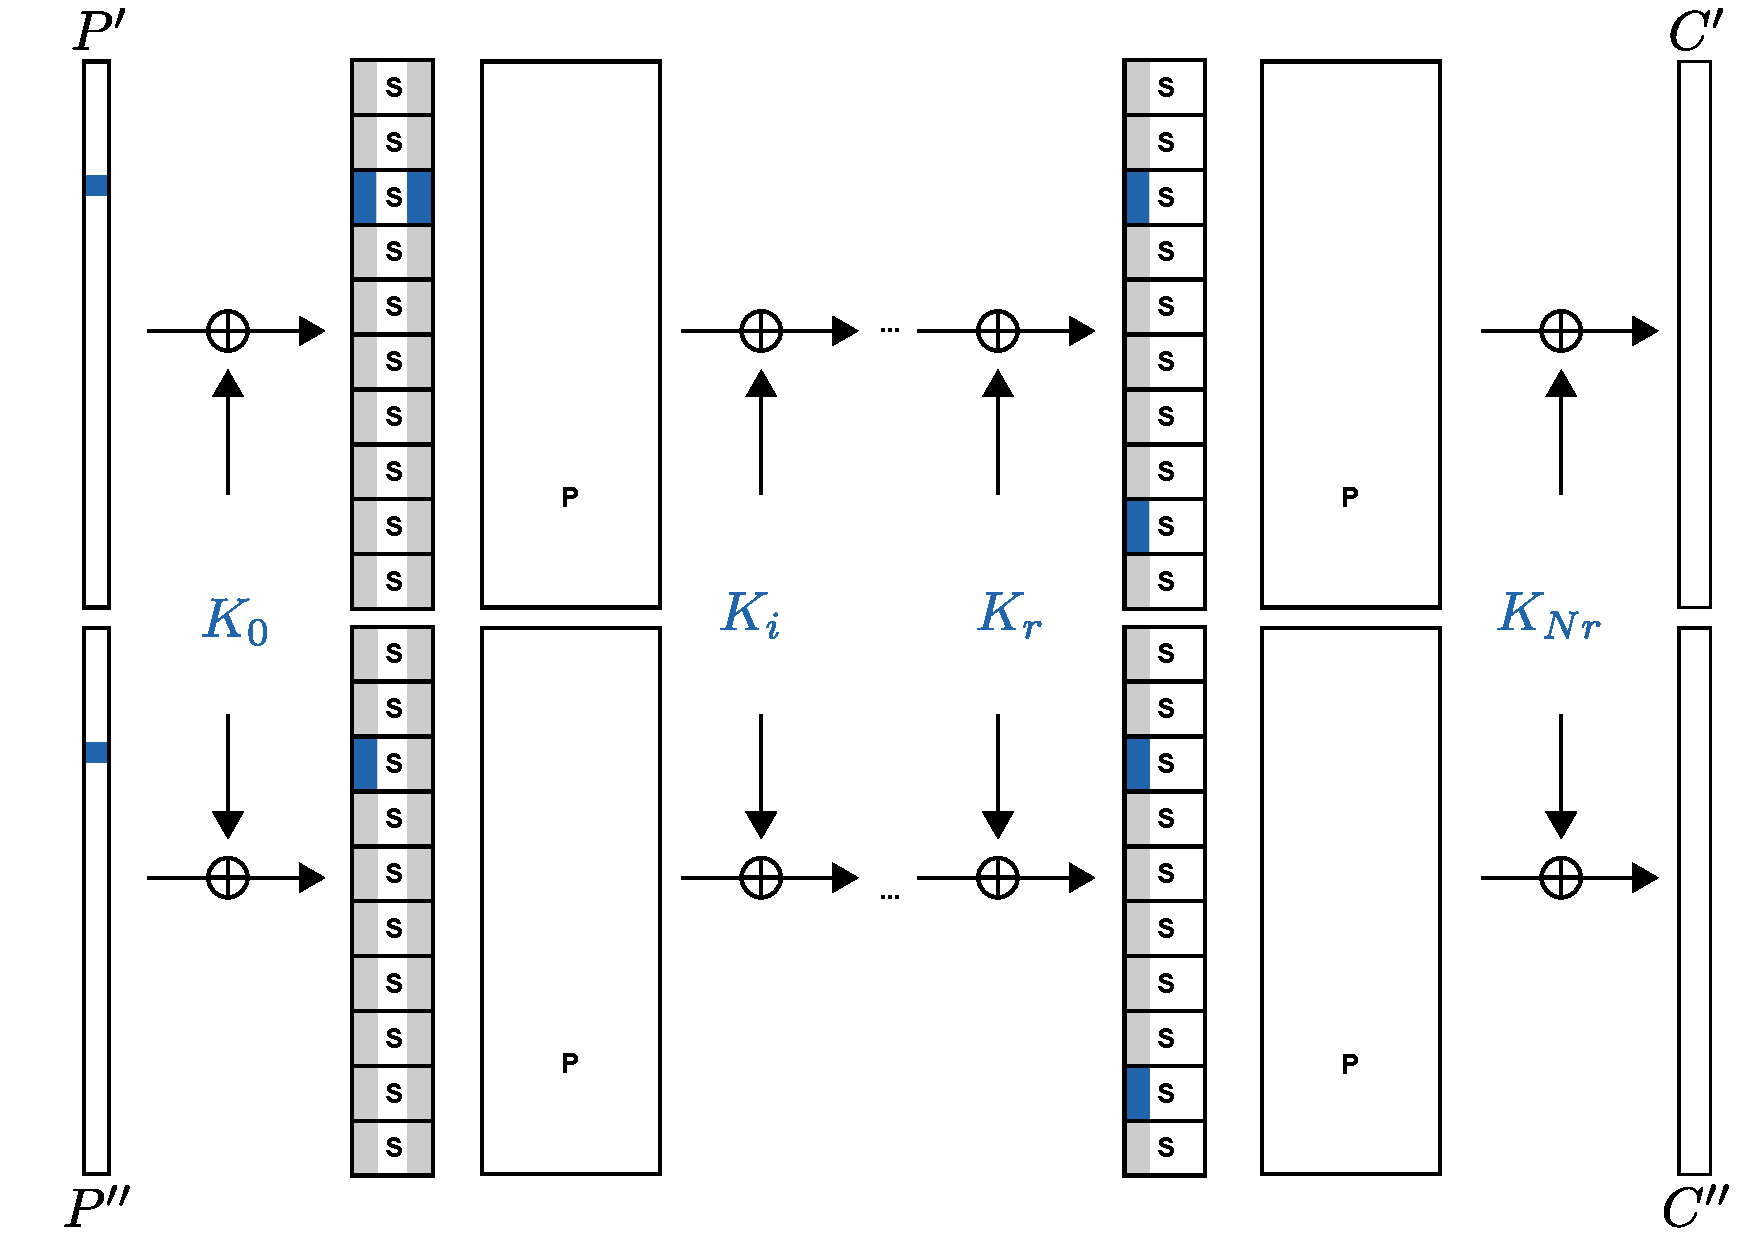
\includegraphics[width=0.8\textwidth]{./attack-a.pdf}
 % attack-a.pdf: 842x595 pixel, 72dpi, 29.70x20.99 cm, bb=0 0 842 595
\end{center}

\framebreak

\begin{center}
 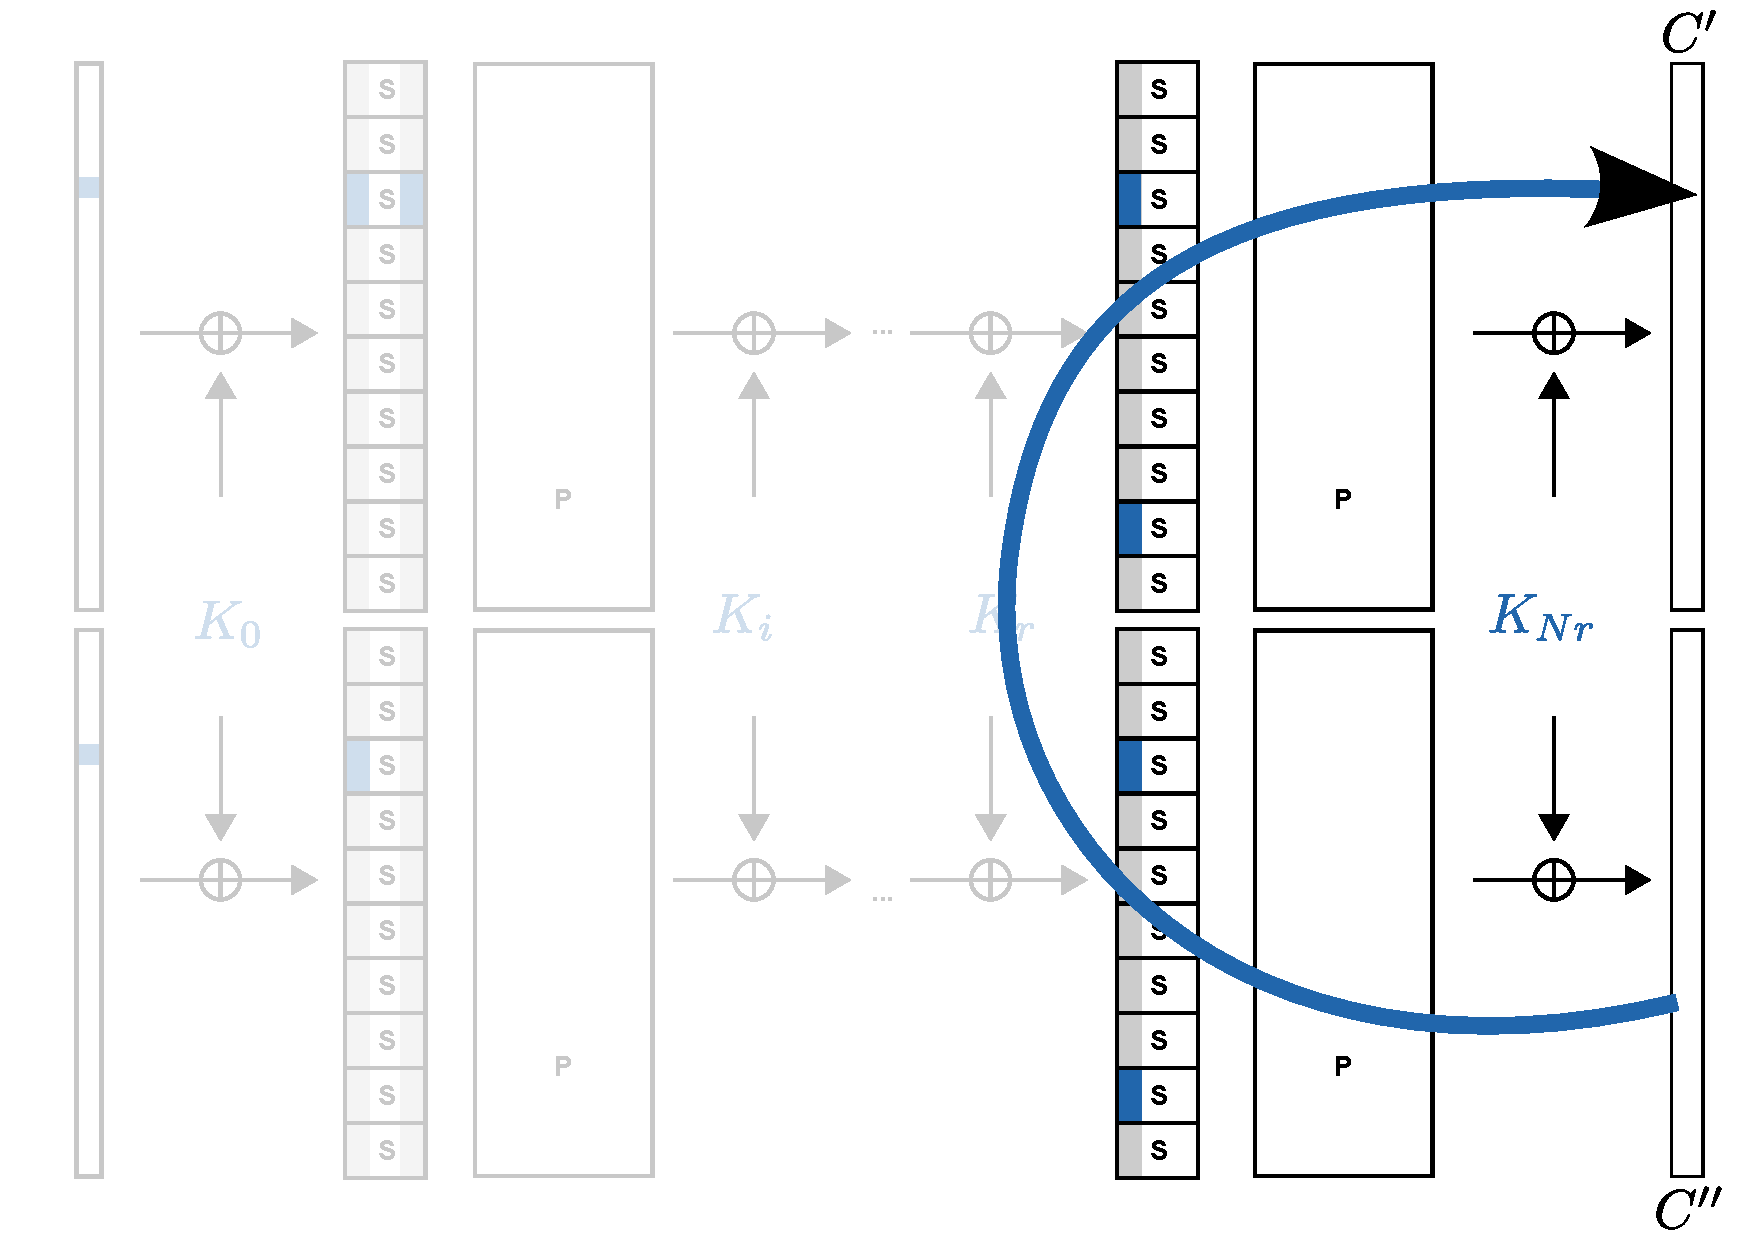
\includegraphics[width=0.8\textwidth]{./attack-c-a.pdf}
\end{center}

\framebreak

\begin{enumerate}
 \item Pick your favourite differential characteristic which holds with probability $p$.
 \item Construct an equation system for two pairs $P'\Rightarrow C'$ and $P'' = P' + \Delta P \Rightarrow C''$.
 \item Add linear equations of the form $X'_{i,j} + X''_{i,j} = \Delta X_{i,j}$  and $Y'_{i,j} + Y''_{i,j} = \Delta Y_{i,j}$ 
 \item Attempt to solve $\mathcal{O}(1/p)$ such systems to get one that has a solution.
\end{enumerate}

\begin{table}[htbp]
\begin{center}
\begin{tabular}{|r|c|r|r|r|}
\hline
Cipher & System & RAM & pairs & time\\
\hline
 \PRESENT-80-14 & C2D 2.33~Ghz & 4~GB & $\approx 2^{44}$ & $2^{72.60}$ CPU cycles \\
 \PRESENT-80-15 & 2.4~Ghz & 64~GB & $\approx 2^{59}$ & $2^{73.79}$ encryptions \\
\PRESENT-128-14 & 2.4~Ghz & 64~GB & $\approx 2^{55}$ & $2^{112.83}$ encryptions\\ 
\PRESENT-128-17 & C2D 2.33~Ghz & 4~GB & $\approx 2^{62}$ & $2^{43.70} \cdot t$ CPU cycles$^*$\\ 
  KTANTAN32-113 & C2D 2.33~Ghz & 4~GB & $\approx 2^{31}$ & $2^{64}$ CPU cycles\\
\hline
\end{tabular}
\end{center}
\end{table}

\vspace{4em}

\begin{small}
* this is a successful attack if $t < 2^{89}$. There is no consensus whether this is plausible.
\end{small}

% \framebreak
% 
% Given a differential characteristic algebraic techniques can also be used to find plaintext/ciphertext pairs (under a chosen key or a free key) which satisfy this characteristic. 
% 
% \vspace{1em}
% 
% For example, it is possible to find right pairs for a 14 round characteristic for \PRESENT-80 which holds with probability $2^{-62}$ in a few hours.

\end{frame}

\begin{frame}
\frametitle{A more general perspective}

We can view the algebraic-differential approach as a special case of:

\begin{itemize}
 \item Find some property which holds with some probability $p$ after $r$ rounds (under some chosen inputs)
 \item Setup a smaller equation system which relates the  property to the output
 \item Attempt to solve the smaller system $\mathcal{O}(1/p)$ times.
 \item For this smaller equation system we have very few ``plaintext-ciphertext'' pairs, hence algebraic techniques seem to fit well.
\end{itemize}

\begin{small}
\begin{thebibliography}{keeloq}
\bibitem{keeloq}
 Nicolas T.\ Courtois, Gregory V. Bard and David Wagner.
 \newblock Algebraic and Slide Attacks on KeeLoq
 \newblock In {\em Fast Software Encryption -- FSE 2008},
 pages  97--115, Berlin, Heidelberg, New York, 2008. Springer Verlag 
\bibitem{gost}
 Nicolas T. Courtois.
 \newblock Security Evaluation of GOST 28147-89 In View Of International Standardisation,
 \newblock In {\em Cryptology ePrint Archive}, Report 2011/211, 2011
\end{thebibliography}
\end{small}
\end{frame}


\begin{frame}
\frametitle{Algebraic Techniques and Integral Cryptanalysis} 

In Integral or Higher-Order Differential Cryptanalysis the attacker encrypts plaintexts with some structure such that the output (after some rounds) also has some (algebraic) structure. 

\vspace{1em}

We can use algebraic techniques find such algebraic relations (cf. Beyond Solving).

\begin{table}[htbp]
\begin{center}
\begin{tabular}{|r|r|r|r|}
\hline
Cipher & Method & \#P & Wall time\\
\hline
\PRESENT-80-5 &  HODC & $5\cdot 2^4$ & $\approx 2^{25.7}$ CPU cycles\\
\PRESENT-80-5 & AHODC & $2^4$ & $\approx 2^{23.3}$  CPU cycles\\
\PRESENT-80-6 &  HODC & $2^{22.4}$ & $\approx 2^{41.7}$  CPU cycles\\
\PRESENT-80-6 & AHODC & $2^{20}$ & $\approx 2^{39.3}$  CPU cycles\\
\PRESENT-80-7 &  HODC & $2^{24.4}$ & $\approx 2^{100.1}$  CPU cycles\\
\PRESENT-80-7 & AHODC & $2^{21.9}$ & $\approx 2^{97.8}$  CPU cycles\\
\hline
KTANTAN32-65 & AHODC & $2^5$& 59004.10~s\\
\hline
\end{tabular}
\end{center}
\end{table}
\end{frame}

\begin{frame}
\frametitle{Algebraic Techniques and Side-Channel Cryptanalysis} 

\begin{itemize}
 \item Side-channel attacks provide information about the internal state of an encryption operation to the attacker.
 \item This information can then be used to recover key information.
 \item Algebraic techniques seem to be natural candidates for this task, because they are good for tracking/propagating dependencies.
\end{itemize}

\begin{small}
\begin{thebibliography}{}
\bibitem{alg-side-channel:eprint}
Mathieu Renauld and Francois-Xavier Standaert.
\newblock Algebraic Side-Channel Attacks.
\newblock In {\em INSCRYPT 2009 -- {I}nformation {S}ecurity and {C}ryptology 5th International Conference}, volume 6151 of {\em Lecture Notes in Computer Science}, pages 393-410, Berlin, Heidelberg, New York, 2009. Springer Verlag.

\bibitem{coldboot}
Martin Albrecht and Carlos Cid.
\newblock Cold Boot Key Recovery by Solving Polynomial Systems with Noise 
\newblock To appear in {\em ACNS 2011 -- 9th International Conference on Applied Cryptography and Network Security}, in {\em Lecture Notes in Computer Science}, Berlin, Heidelberg, New York, 2011. Springer Verlag.
\end{thebibliography}

\end{small}

\end{frame}


\begin{frame}{Questions?}
\begin{center}\textbf{Thank You!}\end{center}
\end{frame}


% \section*{References}
% \begin{frame}[allowframebreaks]
% \frametitle{References}
% \begin{tiny}
% \bibliographystyle{alpha}
% \bibliography{literature}
% \end{tiny}
% \end{frame}
\end{document}
